\documentclass[a4paper,11pt]{article}
\usepackage{jheppub} % for details on the use of the package, please see the JINST-author-manual
\usepackage{lineno}
%\linenumbers
\usepackage{cmupint}
%packages I added after the fact
\usepackage{graphicx} % Required for inserting images
%\usepackage[utf8]{inputenc}
\usepackage[T1]{fontenc}
\usepackage{amsmath}
\usepackage{graphicx}
\usepackage{latexsym,amssymb,lmodern}
\usepackage{float}
\usepackage[colorinlistoftodos]{todonotes}
%\usepackage[a4paper,top=2cm,bottom=2cm,left=2cm,right=2cm,marginparwidth=1.75cm]{geometry}
\usepackage{hyperref}
\usepackage{xcolor}
\usepackage{soul}
\usepackage{cancel}
\usepackage{appendix}
\newtheorem{definition}{Definition}
\newtheorem{theorem}{Theorem}
%\newtheorem{question}{Question}
\newtheorem{importantrelation}{Important Relation}
\newtheorem{question}{Question}
\newcommand{\normord}[1]{:\mathrel{#1}:}
\usepackage{wrapfig}
\usepackage{braket}
\usepackage{physics}
\usepackage{ulem}
\usepackage{cancel}
\usepackage{comment}
%\usepackage{parskip}
%\setlength\parindent{24pt}
\usepackage{enumitem}
%\usepackage{titling}
\usepackage{slashed}
\usepackage{mathscinet}
\usepackage{dsfont} 
\usepackage{simpler-wick}
\usepackage{tikz}
%\usepackage{tikz-feynman}
\usepackage[compat=1.1.0]{tikz-feynman}
%stuff needed to input the github logo
\usepackage{fontawesome5}
\usepackage{xspace}
\usepackage{epigraph}
%\usepackage{fixltx2e}

\makeatletter
\newcommand{\github}[1]{%
   \href{#1}{\faGithubSquare}%
}
\makeatother

%Feynman rule for graviton propagator/legs
\tikzset{graviton/.style={decorate, decoration={snake, amplitude=.4mm, segment length=1.5mm, pre length=.5mm, post length=.5mm}, double}}

\definecolor{green3}{RGB}{44,160,44}

\newcommand{\ac}[1]{\textcolor{green3}{[\textbf{AC:}] #1}}

%\arxivnumber{1234.56789} % if you have one

\title{Everything S-Matrix}

% Collaborations

\author[a]{Alexander Cassem}
\affiliation[a]{Institute of Cosmology, Tufts University, Medford, MA 02155, USA}

% E-mail addresses: only for the corresponding author
\emailAdd{alexander.cassem@tufts.edu}


\abstract{
These are personal notes written in the style of ``lecture notes'' as a way to help organize in my own mind the various topics associated with the S-matrix. These notes are a WORK IN PROGRESS and are not meant to be any definitive source material on the various subjects found within. Please check any results for yourself, as well as the cited source material. 
}



\begin{document}
\maketitle
\flushbottom

\section{A Guide on the Literature}

\ac{Fill-in later, but briefly: trust chapters 1 and 4 of Eden's et al. textbook, and start with Mizera's notes since they are amazing} \cite{Eden:1966dnq,Mizera:2023tfe}.

\section{General Properties of Amplitudes}

\epigraph{The best assumptions are the ones you can't prove.}{\textit{Xi Yin}\\PHY253b}

The title of the section should really be ``\textit{Some} General Properties of Amplitudes,'' since the vastness of the literature on S-matrix results is staggering and ever changing. However, the core results from the 60's and 70's, being re-discovered and re-formulated will never change (only the efficiency of their derivation will). It is these core results that we will be looking at in this section by taking examples of physical setups that can be extended to a more general case. 

\subsection{Examples: $2\rightarrow 2$ Scattering of Identical Massless Scalars}

Consider the $2\rightarrow 2$ scattering amplitude of identical massive scalar particles. The $s$- and $t$-channel can be written in terms of the scattering angle $\theta$ as
\begin{equation}
    s = E^2 = 4(k^2+m^2)\:\:\text{and}\:\: t = -2k^2(1-\cos(\theta))\label{parameterization of s and t channels}.
\end{equation}
We know that the amplitude $A(s,t)$ can be analytically continued away from the physical region $s,t\in\mathbb{R}$ with $s\geq 4m^2-t$ with $t\leq 0$ \footnote{We will still denote the ampliude $\mathcal{A}(s,t)$}. Consider fixing $t<0$ and analytically continue $s$ into the complex plane. This can be see in figure \ref{Complex graph of s}.

\begin{figure}[h]
    \centering
    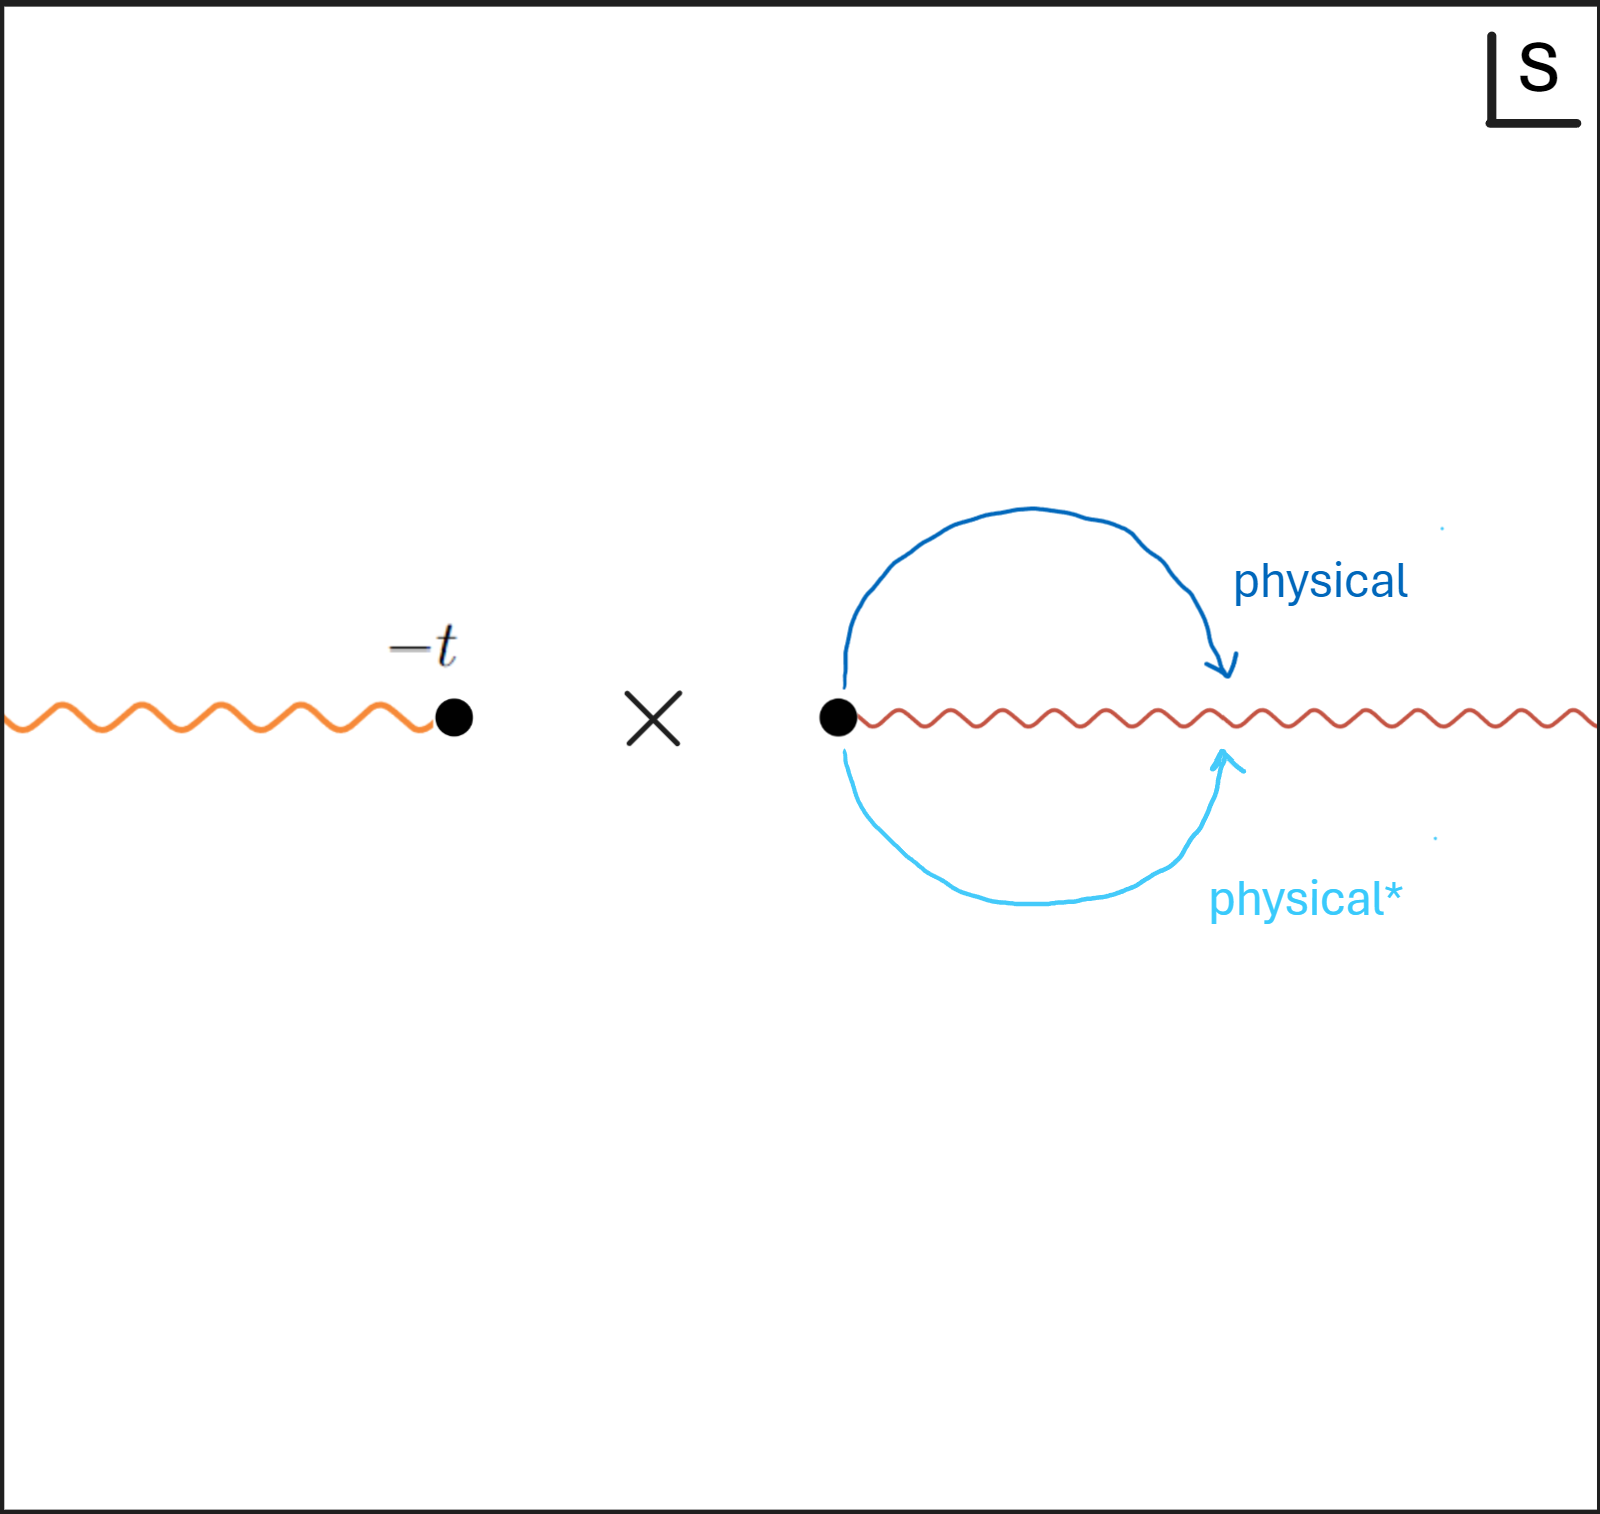
\includegraphics[width=0.5\linewidth]{s channel graph.png}
    \caption{Complex graph of $s$ with branch cuts on $s$-channel and $u$-channel with possible bound state poles denoted as x's.}
    \label{Complex graph of s}
\end{figure}
The \textit{branch cut} on the complex graph of $s$ denotes all the physical states of the theory based on the bounds of $s$. The physical amplitude can be written as
\begin{equation}
    \text{physical amplitude} = \lim_{\epsilon\rightarrow 0^+}A(s+i\epsilon,t)\label{physical amplitude}.
\end{equation}
The limit of \eqref{physical amplitude} is taken such that we analytically continue from above towards the branch cut. If we instead went from $0^-$, then we would have analytically continued from below, finding the complex conjugate of the physical amplitude. Analytically continuing the amplitude $A(s,t)$ is expected to obey the \textit{real analyticity} condition
\begin{equation}
    A(s^*,t^*) = (A(s,t))^*\label{reality condition},
\end{equation}
which can also be thought of as a reality condition \footnote{In perturbation theory,this follows from the reality of coupling constants in the Lagrangian.}. This is the first assumption we will make about the amplitude. The graph in \ref{Complex graph of s} of the $s$-channel is on the \textit{first Riemann sheet} or the \textit{physical sheet}. The cut on the LHS is a $u$-channel cut that starts at $-t$. The crosses denote possible bound state poles. The resonance poles are heinding on the \textit{second sheet} which can be found by translating between momentum to energy \footnote{A classical example from quantum mechanics is when graphing complex $p$ and finding the second sheet by using $p^2/2m = E\implies p = \pm i\sqrt{-2mE}$.}. 

The second assumption we make about the amplitude $A(s,t)$ is that it has a \textit{crossing symmetry}. Crossing symmetry, in terms of the channels, relates the different scattering channels $s,t$, and $u$ to each other via analytically continuing to different regions of $s,t$, and $u$. \ac{Insert Mandelstam graph from \cite{Eden:1966dnq}}. Note that all of the assumptions being made about $A(s,t)$ hold non-perturbatively. 

The third assumption we shall make is about unitarity. \ac{Stopped here.}

\subsection{Comment on Polynomial Boundedness}

\appendix
\section{Derivations of such}
Please always give a title also for appendices.





\acknowledgments

Something something some cool people and such.

\paragraph{Note added.} If we mess something up.


% Bibliography

%% [A] Recommended: using JHEP.bst file
\bibliographystyle{JHEP}
\bibliography{biblio.bib}

%% or
%% [B] Manual formatting (see below)
%% (i) We suggest to always provide author, title and journal data or doi:
%% in short all the informations that clearly identify a document.
%% (ii) please avoid comments such as "For a review'', "For some examples",
%% "and references therein" or move them in the text. In general, please leave only references in the bibliography and move all
%% accessory text in footnotes
%% (iii) Also, please have only one work for each \bibitem.
\begin{comment}
\begin{thebibliography}{99}

\bibitem{a}
Author,
\emph{Title},
\emph{J. Abbrev.} {\bf vol} (year) pg.

\bibitem{b}
Author,
\emph{Title},
arxiv:1234.5678.

\bibitem{c}
Author,
\emph{Title},
Publisher (year).

\end{thebibliography}
\end{comment}
\end{document}
